\section{Support Vector Machines (SVMs)}
\subsection{Introduction}
In this section we are going to deal with a very well known \textbf{supervised learning algorithm}, called \textbf{Support Vector Machine}. We will see that it can be written as an intuitive \textbf{optimization problem} and can be easily extended to work very well with non-linear patterns or in \textbf{high dimensional spaces}.\\

SVM belongs to the class of \textbf{discriminative classifiers} since its goal consists on \textbf{learning the class boundary between the two classes} $y$ starting from features $x$. From now, we'll use $y\in\{-1,1\}$ to denote the class labels. In a 2-dimensions feature space the decision boundary is represented by a straight line, while in general the decision boundary is represented by an \textbf{hyperplane}. An example of decision boundaries in a 2-dimensions feature space is represented in Picture \ref{hyperplanes}.

\begin{figure}[h!]
		\centering
		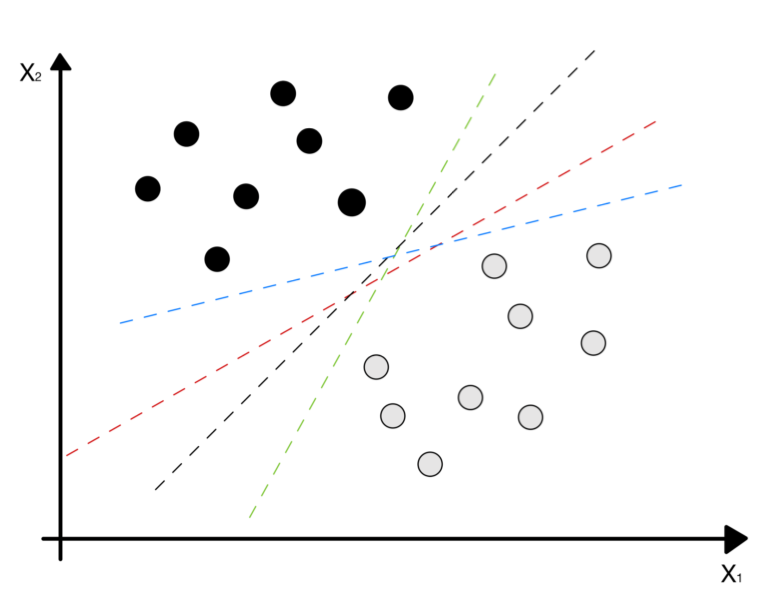
\includegraphics[scale = 1.0]{img/hyperplanes.png}
		\label{hyperplanes}
		\caption{Decision boundaries in a 2-dimensions feature space}
\end{figure}

The data points that are closest to the decision boundary are called \textbf{support vectors}, while the distance between the support vectors along the perpendicular direction to the selected hyperplane is called \textbf{margin}: the hyperplane chosen by SVM is the one that maximize the margin. By choosing this particular hyperplane, the \textbf{misclassification risk} is minimized, since the \textbf{confidence} of the prediction of the model is stronger.

From a mathematical point of view, let's consider a 2-dimension feature space and let's assume labels are such that $y_i \in \{-1, 1\}$. A linear decision boundary $B$ is defined by the equation:
$$
    w^Tx + b = 0
$$
, where $w$ weights the features of $x$, so the objects above $B$ are defined by $w^Tx + b = k'$, where $k' > 0$, while the objects below $B$ are define by $w^Tx  b = k''$, where $k'' < 0$. Let $x_s$ and $x_c$ be the positive and negative support vectors of $B$, we can then rescale $w$ and $b$ such that:

$$
w^Tx_s + b = 1
$$

and 

$$
w^Tx_c + b = -1
$$

Let $d_s$ and $d_c$ be the distances between the support vectors and the decision boundary $B$, then by definition:

$$
d_s = \frac{|w^Tx_s + b|}{||w||} = \frac{|1|}{||w||} = \frac{1}{||w||}
$$

$$
d_c = \frac{|w^Tx_c + b|}{||w||} = \frac{|-1|}{||w||} = \frac{1}{||w||}
$$

Then, the margin $d$ is defined as:

$$
d = d_s + d_c = \frac{2}{||w||}
$$

\begin{figure}[h!]
		\centering
		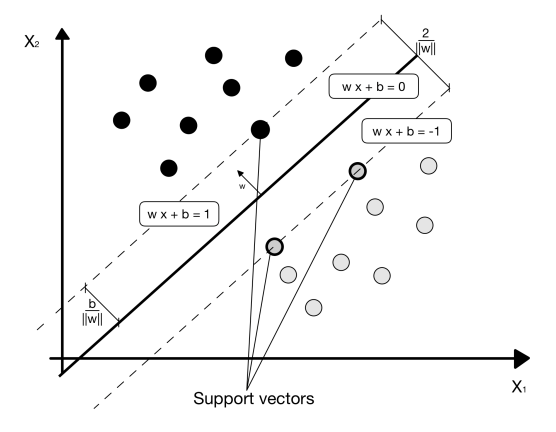
\includegraphics[scale = 1.0]{img/sv.png}
		\label{svm}
		\caption{Geometric representation of SVM}
\end{figure}

Thus, given a training set $L = \{ (x_1, y_1), .., (x_N, y_N) \}$, learning an SVM can be formulated as an optimization problem: indeed, the goal of SVM is to \textbf{maximize} $\frac{2}{||w||_2}$ or, equivalently, \textbf{minimize} $\||w||_2$. Finally, we can describe the SVM (binary) classification problem as:

\begin{equation}\label{eq_svm1}
\begin{aligned}
\max_{w} \quad & \frac{2}{||w||}\\
\textrm{s.t.} \quad & y_{i}(w^Tx_{i}+b) - 1 \geq 0 \quad \forall i = 1,..,N\\ \\
\end{aligned}
\end{equation}

or, equivalently

\begin{equation}\label{eq_svm2}
\begin{aligned}
\min_{w} \quad & \frac{1}{2} ||w||^2\\
\textrm{s.t.} \quad & y_{i}(w^Tx_{i}+b) - 1 \geq 0 \quad \forall i = 1,..,N\\ \\
\end{aligned}
\end{equation}

Since the objective functions in \ref{eq_svm1} and \ref{eq_svm2} are quadratic, and the constraints are linear in $w$ and $b$, this is known to be a \textbf{convex optimization problem}, which means that there exists a unique minimum! This unique minimum corresponds to the \textbf{optimal margin classifier}. 

\subsection{Lagrangian and duality}
\subsubsection{Unconstrained optimization}
Suppose we want to find the maximum of the following 2-dimensions function:

$$
f(x,y) = 1 - x^2 - y^2
$$

From calculus we know that the solution must be found among the points $(x,y)$ where the gradient $\nabla f(x,y)$ vanishes, i.e. in the so-called \textbf{stationary points}:

$$
\frac{\partial f(x,y)}{\partial x} = -2x = 0
$$

and

$$
\frac{\partial f(x,y)}{\partial y} = -2y = 0
$$

In this sense, the solution is given by $x = 0$ and $y = 0$.

\subsubsection{Constrained optimization}
Suppose now that the points $(x,y)$ have to lie on the straight line of equation $x + y = 1$, i.e. we want to solve the following constrained optimization problem:

\begin{equation*}\label{eq_svm2}
\begin{aligned}
\max \quad & 1 - x^2 - y^2\\
\textrm{s.t.} \quad & x + y - 1 = 0\\ \\
\end{aligned}
\end{equation*}

Our goal is now to define a method for transforming the constrained optimization problem into an unconstrained one. To this end, we define a new function $L(x,y,\lambda)$, called the \textbf{Lagrangian} as follows:

$$
L(x,y,\lambda) = 1 - x^2 - y^2 + \lambda(x + y - 1)
$$

, where $\lambda \neq 0$ is called a \textbf{Lagrangian multiplier}, and looks for points $(x,y,\lambda)$ where the gradient $\nabla L$ vanishes. Notice that in $L$ we now have as many new variables as the constraints we have. If we apply this method to example, we get the following system of linear equations:

$$
\frac{\partial L(x,y,\lambda)}{\partial x} = -2x + \lambda = 0
$$

$$
\frac{\partial L(x,y,\lambda)}{\partial y} = -2y + \lambda = 0
$$

$$
\frac{\partial L(x,y,\lambda)}{\partial \lambda} = x + y - 1 = 0
$$

, from which we get the solution $x = y = \frac{1}{2}$

\subsubsection{General case}
More generally, given the following optimization problem:

\begin{equation*}\label{eq_svm2}
\begin{aligned}
\max \quad & f(x)\\
\textrm{s.t.} \quad & g_1(x) \geq 0 .. g_m(x) \geq 0  \\
\textrm{    } \quad & h_1(x) = 0 .. h_n(x) = 0
\end{aligned}
\end{equation*}

, where we have $m$ inequality constraints and $n$ equality constraints, the Lagrangian is defined as:

$$
L(x, \Lambda, M) = f(x) + \sum_{i = 1}^m \lambda_i g_i(x) + \sum_{j = 1}^n \mu_j h_j(x)
$$
, where $\Lambda = (\lambda_1, .., \lambda_m)^T$ and $M = (\mu_1, .., \mu_n)^T$ are vectors of Lagrange multipliers corresponding to inequality and equality constraints, respectively.

In this case we need to impose the conditions $\lambda_i \geq 0$ and $\lambda_i g_i(x) = 0$ for all $i = 1,..,m$

The \textbf{intuition} behind the \textbf{equality constraints} is the following one: at any point $x$ in the constraint surface, $\nabla g(x)$ is normal to the surface, from the properties of the gradient. Then, if $x$ is also a maximizer of $f$, $\nabla f(x)$ must be orthogonal to the surface too (otherwise we could increase the value of $f$ with another point), so we have that:

$$
\nabla f(x) = - \lambda \nabla g(x)
$$

, with $\lambda \neq 0$.

\begin{figure}[h!]
		\centering
		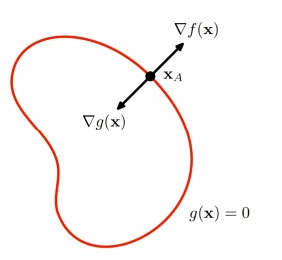
\includegraphics[scale = 1.5]{img/equality constraints intuition.jpg}
		\label{svm}
		\caption{Equality constraints}
\end{figure}

The \textbf{intuition} behind the \textbf{inequality constraints} is the following one. We have two cases:

\begin{itemize}
    \item The solution is in the interior, i.e. $g(x) > 0$: in this case the stationary point condition implies $\nabla f(x) = 0$, which corresponds to the case $\lambda = 0$;
    \item The solution is on the boundary, i.e. $g(x) = 0$: this is analogous to the previous case, but this time the sign of $\lambda$ is crucial: hence $\nabla f(x) = -\lambda \nabla g(x)$, with $\lambda > 0$.
\end{itemize}

For either of these cases we have $\lambda g(x) = 0$

\begin{figure}[h!]
		\centering
		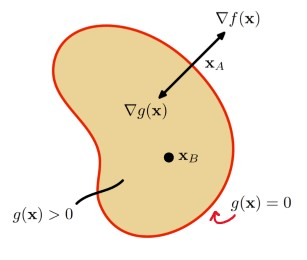
\includegraphics[scale = 1.5]{img/inequality constraints intuition.jpg}
		\label{svm}
		\caption{Inequality constraints}
\end{figure}

Notice that if we want to minimize, rather than maximize, $f(x)$, the Lagrangian multipliers have to be non-positive, or simply change the sign of the corresponding term in the Lagrangian.

\subsubsection{Duality}
Consider the following optimization problem with inequality constraints, called the \textbf{primal}:

\begin{equation*}\label{duality}
\begin{aligned}
\min \quad & f(x)\\
\textrm{s.t.} \quad & g_1(x) \geq 0 .. g_m(x) \geq 0  \\
\end{aligned}
\end{equation*}

with optimal value $p^*$, and consider its Lagrangian:

$$
L(x, \lambda_1, .., \lambda_m) = f(x) - \sum_{i = 1}^m \lambda_i g_i(x)
$$

Notice that the Lagrangian has a minus sign since the problem is a minimization.

Given $\lambda_1, .., \lambda_m \geq 0$, we define the (Lagrangian) \textbf{dual function} as:

$$
\phi(\lambda_1, .., \lambda_m) = \inf_x L(x, \lambda_1, .., \lambda_m)
$$

It's easy to see that $\phi(\lambda_1, .., \lambda_m) \leq p*$, i.e. the optimal value of the previous problem is an upper bound of this second problem.

The problem 

\begin{equation*}\label{eq_svm2}
\begin{aligned}
\max \quad & \phi(\lambda_1, .., \lambda_m)\\
\textrm{s.t.} \quad & \lambda_1, .., \lambda_m \geq 0  \\
\end{aligned}
\end{equation*}

is called the (Lagrangian) \textbf{dual} of problem \ref{duality}.

\paragraph{Weak duality:} if $p^*$ is a solution of the primal and $d^*$ is a solution of its dual, then:

$$
d^* \leq p^*
$$

The quantity $d^* - p^* \leq 0$ is called \textbf{duality gap}.

\paragraph{Strong duality:} if the function $f$ of the primal is convex (and so are all $-g_i$), then

$$
p^* = d^*
$$
, i.e. the solution of the dual (which is simpler) is the same as the solution of the primal.

\paragraph{Wolfe duality:} the \textbf{Wolfe dual} is defined as:

\begin{equation*}\label{eq_svm2}
\begin{aligned}
\max_{x,\Lambda} \quad & L(x,\Lambda)\\
\textrm{s.t.} \quad & \nabla_x L(x,\Lambda) = 0  \\
\textrm{    } \quad & \Lambda \geq 0  \\
\end{aligned}
\end{equation*}

, where $\Lambda = (\lambda_1, .., \lambda_m)$.

Assume that functions $f$ and $-g_i$ are convex (and continuously differentiable): if $x^*$ is a solution of the \textbf{primal problem}, then there exists a \textbf{vector of Lagrangian multipliers} $\Lambda^*$ s.t. $(x^*, \Lambda^*)$ is a \textbf{solution} of the \textbf{Wolfe dual}, and the duality gap is 0.

\subsubsection{Dual representation of SVM}
In order to solve constrained problem 

\begin{equation}\label{eq_svm2}
\begin{aligned}
\min_{w} \quad & \frac{1}{2} ||w||^2\\
\textrm{s.t.} \quad & y_{i}(w^Tx_{i}+b) - 1 \geq 0 \quad \forall i = 1,..,N\\ \\
\end{aligned}
\end{equation}

we introduce the concept of \textbf{Lagrange multipliers}. Using the \textbf{Lagrange} function with $N$ Lagrange multipliers $\Lambda = (\lambda_1,\dots,\lambda_N)$ (one for each constraint) it is possible to rewrite the correspondent optimization problem, with parameters $w$ and $b$, into an identical one but with parameters $(\lambda_1,\dots,\lambda_N)$. Taking advantage of the \textbf{dual representation}, that allows to convert an original min/max problem into another one which is equivalent but with max/min formulation, we can write the \textbf{new optimization problem}as follows:

\begin{equation}
\quad L(w,b,\Lambda) = \frac{1}{2}||w||^2 - \underbrace{\sum_{i = 1}^{N}\lambda_i[y_i(w^Tx_i+b)-1]}_{\text{Sum of constraints}}\\
\end{equation}
, where $\Lambda = (\lambda_1, .., \lambda_N)$ is the vector if Lagrange multipliers.

The goal now is to find a \textbf{function} \textbf{parameterized} only by \textbf{Lagrangian multipliers}. Setting the derivatives of $L(w,b,\Lambda)$ to zero we get:

$$\frac{\partial L(w,b,\Lambda)}{\partial w} = w- \sum_{i = 1}^{N}\lambda_iy_ix_i = 0 \qquad \implies \qquad w = \sum_{i = 1}^{N}\lambda_iy_ix_i$$

$$
\frac{\partial L(w,b,\Lambda)}{\partial b} =\sum_{i = 1}^{N}\lambda_iy_i = 0 
$$

Eliminating $w$ and $b$ from $L(w,b,\Lambda)$ using these conditions we obtain a new formulation of the optimization problem expressed with only Lagrangian multipliers:

\begin{equation*}
\begin{aligned}
&\text{max }\quad L_D(\lambda_1,\dots,\lambda_N) = \sum_{i = 1}^{N}\lambda_i - \frac{1}{2}\sum_{i = 1}^{N}\sum_{j = 1}^{N}\lambda_i\lambda_jy_iy_jx_i^Tx_j\\
&\text{s.t.} \quad \sum_{i = 1}^{N}\lambda_iy_i= 0 \qquad \lambda_i \geq 0, \forall i = 1,\dots,N\\
\end{aligned}
\end{equation*}

On the one hand, in this case we have a number of variables which is equal to the number of examples in the training set, i.e. we have much \textbf{more variables}. However, it can be noticed that the \textbf{training vectors} only appear as \textit{dot products}, and the advantage of using this formulation is that only \textbf{support vectors} will have \textbf{Lagrange multipliers} such that $\lambda_i > 0$ and the \textbf{others} will be essentially \textbf{equal to zero} (sparse solution). The \textbf{SVM complexity} is only given by the \textbf{support vectors} (which are much less than the number of examples in the training set). Now the \textbf{maximum margin hyperplane} is given by:

$$\sum_{i = 1}^{m} y_i \lambda_ix_i^Tx+b = 0$$

If $\Lambda = (\lambda_1,\dots, \lambda_N)$ is the solution of the dual optimization problem, then:
\begin{itemize}
	\item The \textbf{weight vector} of the maximum margin hyperplane is:
	$w = \sum_{i = 1}^{N} y_i\lambda_ix_i$
	\item The corresponding \textbf{discriminant function} (separating hyperplane) is:
	$$f(x) = w^Tx+b =  \sum_{i = 1}^{N} y_i\lambda_ix_i^Tx_i + b$$
	\item The \textbf{linear SVM classifier} $g: \mathbb{R}^n \rightarrow \{-1,1\}$ is:
	$$g(x) = \text{sign}(w^Tx+b) = \text{sign} (\sum_{i = 1}^{N} y_i\lambda_ix_i^Tx_i + b)$$
\end{itemize}
For support vectors we have:
$$y_i(\sum_{i = 1}^{N} y_i\lambda_ix_i^Tx_i + b) = \gamma$$
, and for simplicity we consider $\gamma = 1$.
Since SVM is affected only by support vectors we can derive:
$$b = \frac{1}{|SV|}\sum_{i\in SV}\Large(y_i-\sum_{j=1}^{N}y_j\lambda_jx_j^Tx_i\Large)$$
where \textbf{SV} is the \textbf{set of support vectors}.

\subsubsection{SVM error function}
The generic loss function adopted for training a support vector machine is the \textbf{Hinge loss function}. 
$$L_{\text{hinge}} = \max \{0, 1- y_if(x_i)\}$$
\image{img/hingeloss.png}{Hinge loss function.}{0.45}
$$E = \sum\limits_{i=1}^N\max\{0,1-y_if(x_i)\}+\frac{1}{2}\sum\limits_{j = 1}^dw_j^2$$

, where

\begin{itemize}
	\item $\sum\limits_{i=1}^N\max\{0,1-y_if(x_i)\}$ represents the hinge loss function over all data points;
	\item $\frac{1}{2}\sum\limits_{j = 1}^dw_j^2$ is proportional to the inverse of the margin.
\end{itemize}
Notice that the hinge loss function is not differentiable on $1$, we can't apply the gradient descent procedure. The solution of this problem consists on using \textbf{quadratic programming (QP)} algorithms, since $E$ is a quadratic function with linear constraints.


\subsubsection{SVMs and the VC dimension}
\paragraph{Theorem (Vapnik)} Consider \textbf{hyperplanes} $w^Tx+b= 0$ in canonical form, that is such that:
$$\min\limits_{1\leq i \leq N}|w^Tx_i+b| = \gamma = 1$$
Then the \textbf{set of decision functions} $g(x) = sgn(w^Tx+b)$ (i.e. of SV classifiers) that satisfy the \textbf{constraint} $||w|| < \gamma$ has a \textbf{VC dimension} $h$ satisfying:
$$h \leq R^2\gamma^2$$
where $R$ is the \textbf{smallest radius} of the sphere around the origin containing all the \textbf{training points}. Note that dropping the condition $||w|| < \gamma$ leads to a VC dimension equal to $n+1$. Hence, the constraint allows us to work in high-dimension spaces. \\
From the previous theorem and from:
$$R(f) \leq R_{\text{emp}}(f) + \sqrt{\frac{h(\log(\frac{2n}{h})+1)-\log(\frac{\sigma}{4})}{n}}$$
we have:
\begin{itemize}
	\item By \textbf{maximizing the margin}, or equivalent by \textbf{minimizing} $||w||$, we are in fact \textbf{minimizing} the \textbf{VC dimension} of the SVM;
	\item The \textbf{minimization of the expected} risk depends on both \textbf{minimizing} the \textbf{empirical risk} and the \textbf{confidence interval};
	\item The \textbf{confidence interval} depends mainly on the \textbf{ratio} $\frac{h}{n}$;
	\item The \textbf{SVM algorithm minimizes} both the \textbf{empirical risk} and the \textbf{confidence interval};
	\item The \textbf{SVM} directly implements the \textbf{structural risk minimization principle}.
\end{itemize}

\subsection{How to manage outliers: soft margins}
One of the problems of SVMs is to make decisions in presence of \textbf{outliers}.
\image{img/outlierSVM1.png}{Outliers effects on an SVM.}{0.55}
The previous image shows the effect that a single outlier can have. We can make only one of the following choices: \textbf{correctly classify} the outlier, thus improving the \textbf{accuracy} of the classifier and produce a \textbf{smaller margin}, or leave the outlier \textbf{mis-classified}, thus diminishing the accuracy but resulting in a \textbf{larger margin}. The strategy which is commonly adopted is the \textbf{second one}, as the first one would find \textbf{decision boundaries} that work well on the training set, but do \textbf{not provide optimal performance during testing}. 

In order to reduce the effects of mis-classification we adopt some \textbf{slack variables}, useful for allowing some errors in the boundary.
\image{img/outliersSVM.png}{Outliers effects on an SVM with slack variables.}{0.55}
These \textbf{variables} indicate \textbf{how} much we can \textbf{violate} the \textbf{constraints} of SVM, and a slack variable is added for each of the points in the dataset. 

Now the optimization problem can be reformulated as follows:
\begin{equation*}
\begin{aligned}
&\text{min} \quad \frac{1}{2}||w||^2+ C\sum\limits_{i = 1}^N\xi_i\\
&\text{s.t.} \quad y_i(w^Tx_i-b)\geq 1 - \xi_i\\
&\text{s.t.} \quad \xi_i \geq 0 \qquad i = 1,\dots,N
\end{aligned}
\end{equation*}

The only parameter \textit{C} controls the \textbf{tradeoff} between the \textbf{accuracy} with respect to the training data and the \textbf{maximization} of the \textbf{margin}. It can be interpreted also as a \textbf{regularization term}:
\begin{itemize}
	\item \textbf{small} $C$ allows constraints to be easily ignored \textit{(large margin)}.
	\item \textbf{large} $C$ makes constraints hard to ignore \textit{(narrow margin)}.
	\item $C = \infty$ enforces \textbf{all constraints} \textit{(hard margin)}.
\end{itemize}

The \textbf{dual representation} of the problem can be reformulated as follows:

\begin{equation*}
\begin{aligned}
&\text{max }\quad L_D(\lambda_1,\dots,\lambda_N) = \sum_{i = 1}^{N}\lambda_i - \frac{1}{2}\sum_{i = 1}^{N}\sum_{j = 1}^{N}\lambda_i\lambda_jy_iy_jx_i^Tx_j\\
&\text{s.t.} \quad \sum_{i = 1}^{N}\lambda_iy_i= 0 \qquad \forall i = 1,\dots,N\\
&\text{s.t.} \quad 0 \leq \lambda_i \leq C \qquad \forall i = 1,\dots, N
\end{aligned}
\end{equation*}

The hyperplanes whose weight vectors solve this quadratic optimization problem are called the \textbf{soft margin hyperplanes}. The soft-margin optimization problem is equivalent to that of the maximum margin hyperplanes with the additional constraint $\lambda_i \leq C$ (box constraints). This \textbf{approach} \textbf{limits} the effect of the \textbf{outliers} (for which $\lambda_i$ tends to be large).

\image{img/hinglosswithslack.png}{Hinge loss function with slack variables.}{0.8}

\image{img/csvm.png}{Effect of C on the decision boundary.}{0.7}


\subsection{Nonlinear SVM's: Kernel trick}
Thus far we worked with the assumption that the space is \textbf{linearly separable}, but SVMs allow the usage of a strategy, called \textbf{kernel trick}, for learning a possible separating hyperplane in a \textbf{new space}.
As a matter of fact, in some cases it could be interesting to try and classify points in a \textbf{transformation of the original space}. The classic situation in which we may apply the kernel trick is when \textbf{data points} are \textbf{not} \textbf{linearly separable} in the original space. 

\begin{figure}[h!]
		\centering
		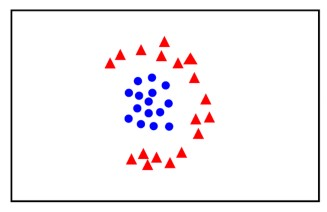
\includegraphics[scale = 1.5]{img/nonlinear svm.jpg}
		\label{svm}
		\caption{Non-linear problem}
\end{figure}

The idea is to define a function $\phi(x)$ that applies a \textbf{mapping} of a \textbf{feature vector} to \textbf{another} one. The SVM algorithm, instead of considering vector $x$, learns using the transformed vector $\phi(x)$. A \textbf{kernel} function is nothing but an \textbf{inner product} between feature mappings of $\phi$:
$$K(x,z) = \phi(x)^T\phi(z)$$

\begin{exmp}
The following Picture represents an example of possible mapping of the data points into a new space in order to make them linearly separable.
    \begin{figure}[h!]
		\centering
		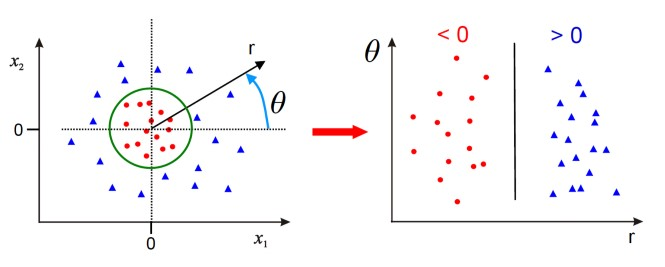
\includegraphics[scale = 1.5]{img/example of transformation.jpg}
		\label{svm}
		\caption{Example of mapping}
\end{figure}

As we can see, data is now represented in polar coordinates (each point is defined by the radius $r$ and the angle $\theta$), so the points are now linearly separable. In this case $\phi : (x_1, x_2)  \in \mathbb{R}^2 \to (r,\theta) \in \mathbb{R}^2$, so in this case we did not project the feature in a larger dimensionality vector.

\end{exmp}

\paragraph{Cover's Theorem} \textit{A complex pattern-classification problem cast in a high-dimensional space non-linearly is more likely to be linearly separable than in a low-dimension space.}\\

In other words, this theorem states that if we map the points of a problem which is not linearly separable into a higher dimensional space, then the problem is more likely to be linearly separable. The \textbf{power} of\textbf{ SVM's} resides in the fact that they represent a \textbf{robust} and \textbf{efficient} \textbf{implementation} of Cover's \textbf{theorem}.

In general, nonlinear SVM's operate in two stages:

\begin{enumerate}
    \item Perform a (typically implicit) \textbf{non-linear mapping} $\phi$ of the feature vector $x$ onto a high-dimensional space that is hidden from the inputs or the outputs. This represents the most difficult step;
    \item Construct an \textbf{optimal separating} \textbf{hyperplane} using SVM's in the high-dimensional space.
\end{enumerate}

We recall that in the dual representation of SVM's the inputs appears only in a \textbf{dot-product form}, i.e.

\begin{equation*}
\begin{aligned}
&\text{max }\quad L_D(\lambda_1,\dots,\lambda_N) = \sum_{i = 1}^{N}\lambda_i - \frac{1}{2}\sum_{i = 1}^{N}\sum_{j = 1}^{N}\lambda_i\lambda_jy_iy_jx_i^Tx_j\\
&\text{s.t.} \quad \sum_{i = 1}^{N}\lambda_iy_i= 0 \qquad \forall i = 1,\dots,N\\
&\text{s.t.} \quad 0 \leq \lambda_i \leq C \qquad \forall i = 1,\dots, N
\end{aligned}
\end{equation*}

and the discriminant function obtained from the solution is:
$$f(x) = \sum\limits_{i = 1}^Ny_i\lambda_ix_i^Tx +b$$

Now we can \textbf{replace} the simple \textbf{inner product} with a \textbf{kernel function} in order to learn in a different feature space, which in some cases could be more efficient. There is a restriction on the function $K$: it must satisfy the following \textbf{property} (called Mercer's condition) in order to be considered a \textbf{valid kernel}:
$$K(x,z) = \phi(x)^T\phi(z) \qquad \forall x, z \in S$$

In this sense, suppose we first \textbf{mapped} the data to some other (possibly infinite dimensional) Euclidean space, using a mapping:
$$x \rightarrow \phi(x) \qquad K(x,y) = \phi(x)^T\phi(y)$$

\begin{equation*}
\begin{aligned}
&\text{max }\quad L_D(\lambda_1,\dots,\lambda_N) = \sum_{i = 1}^{N}\lambda_i - \frac{1}{2}\sum_{i = 1}^{N}\sum_{j = 1}^{N}\lambda_i\lambda_jy_iy_jK(x_i,x_j)\\
&\text{s.t.} \quad \sum_{i = 1}^{N}\lambda_iy_i= 0 \qquad \forall i = 1,\dots,N \\
&\text{s.t.} \quad 0 \leq \lambda_i \leq C \qquad \forall i = 1,\dots,N
\end{aligned}
\end{equation*}

Now, the \textbf{discriminant function} is:

$$f(x) = \sum\limits_{i = 1}^Ny_i\lambda_iK(x_i, x) +b$$

Note that now is \textbf{not necessary} to compute $\phi(x)$.

There exist many kernels, for instance:
\begin{itemize}
	\item \textbf{Linear}: $K(x_i,x_j) = x_i^Tx_j$, which performs an identity mapping;
	\item \textbf{Polynomial kernel}: $K(x_i,x_j) = (1 + x_i^Tx_j)^d$, for any $d > 0$;
	\item \textbf{Gaussian kernel} (RBF): 
	$K(x_i, x_j) = \exp\left(-\frac{\|x_i - x_j\|^2}{2\sigma^2}\right)$, for any $\sigma > 0$.
\end{itemize}
\begin{figure}[!h]
	\begin{minipage}[t]{0.5\linewidth}
		\centering
		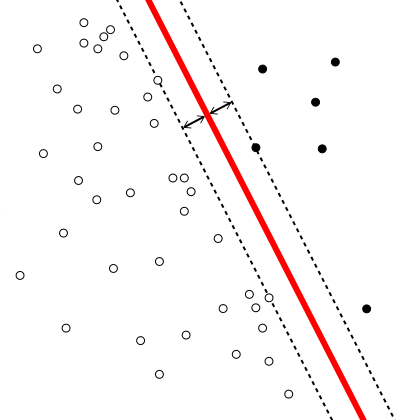
\includegraphics[width=0.41\textwidth]{img/Linear_Kernel_Machine.png}
		\caption{Linear kernel}
		\label{f1}
	\end{minipage}
	\hspace{0.1cm}
	\begin{minipage}[t]{0.5\linewidth} 
		\centering
		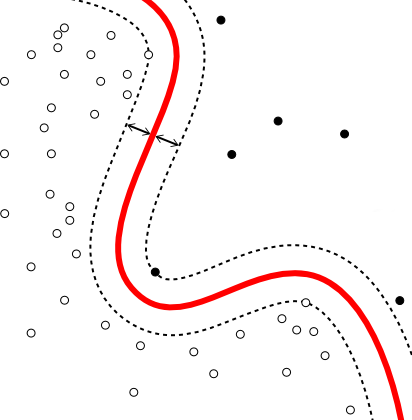
\includegraphics[width=0.41\textwidth]{img/Poly_Kernel_Machine.png}
		\caption{Polynomial kernel}
		\label{f2}
	\end{minipage}        
\end{figure} 
\image{img/RBF_Kernel.png}{Gaussian kernel}{0.3}

\subsection{Multi-class problems}
Thus far we have only discussed about the application of an SVM using \textbf{two labels} $y \in\{-1,1\}$. In real cases, however, we can have more than two classes and we might need to develop an SVM capable of assigning input vectors to one in $K$ \textbf{classes}. In other words, we have to find a decision rule that divides the input space into $K$ \textbf{decision regions} separated by decision boundaries. 
\image{img/multiclass.png}{Decision boundaries for 3 classes.}{0.3}
We can apply two distinct strategies:
\begin{itemize}
	\item \textbf{One-vs-rest classifiers}: train $K-1$ classifiers, \textbf{each} of which solves a \textbf{two-class problem} of separating points in a particular class from points not in that class.
	
	\item \textbf{One-vs-one classifiers}, train $K(K-1)/2$ \textbf{binary classifiers}, one for every possible pair of classes.
	
\end{itemize}

\begin{figure}[!h]
	\begin{minipage}[t]{0.5\linewidth}
		\centering
		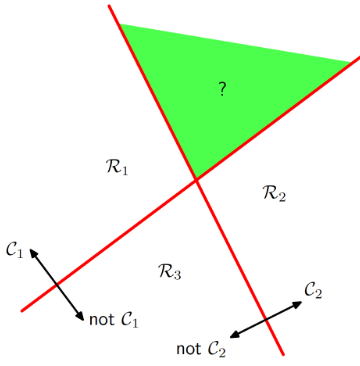
\includegraphics[width=0.51\textwidth]{img/onevsrest.png}
		\caption{One-vs-the-rest classifiers.}
	\end{minipage}
	\hspace{0.1cm}
	\begin{minipage}[t]{0.5\linewidth} 
		\centering
		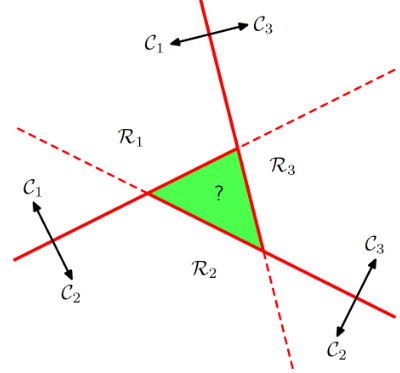
\includegraphics[width=0.51\textwidth]{img/onevsone.png}
		\caption{One-vs-one classifier.}
	\end{minipage}        
\end{figure} 

Note that in the first case the green area denotes a region in which the points are both in $C_1$ and in $C_2$, while in the second case the points in the green area are in $C_1$, $C_2$ and $C_3$ at the same time. Thus, in both cases we have contradictory results. The \textbf{classical approach} consists on training $K$ \textbf{one-vs-rest classifiers} and then the classification is done choosing the \textbf{class} with the ``\textbf{most positive}'' score.

\image{img/learnKclasses.png}{Decision boundaries on typical approaches.}{0.5}

\subsection{Advantages and disadvantages}
Among the \textbf{advantages} we can find:

\begin{itemize}
    \item SVM works relatively \textbf{well} when there is a \textbf{clear margin} of separation between classes;
    \item SVM is\textbf{ more effective} in \textbf{high dimensional spaces} and is relatively memory efficient;
    \item SVM is \textbf{effective} in cases where the \textbf{dimensions are greater than the number of samples}.
\end{itemize}

On the other hand, the \textbf{disadvantages} are:

\begin{itemize}
    \item SVM algorithm is \textbf{not suitable} for \textbf{large data sets};
    \item SVM does \textbf{not perform very well} when the data set has more \textbf{noise} i.e. target classes are overlapping. In cases where the number of features for each data point exceeds the number of training data samples, the SVM will underperform.
    \item As the support vector classifier works by putting data points, above and below the classifying hyperplane there is \textbf{no probabilistic explanation} for the classification.
\end{itemize}